\section{Refinement Application: Docker Documentation}
\label{sec:application}
\subsection{Question Sets and Selection}
Fifteen complex tasks combine seven existing tasks with eight source-grounded
model proposals from previously unrepresented areas, yielding 73 author-reviewed
requirements. Separately, 111 of 142 FAQs had LLM-verified baseline support.
Both sets were frozen before refinement and withheld from the editor.
Whole-page rejudgment leaves 105 FAQs supported in every arm for primary
retrieval comparisons; answer scoring retains all 111.

\subsection{Refinement Morphology and Controls}
The application compares leaf-and-trunk refinement (LT) with uninformed refinement (R0).
LT keeps task-specific steps in leaves linked to shared
procedures, prerequisites and context in trunks.
Leaves have outgoing links; these content roles need not form a rooted tree.
Nam et al. observed experienced-user clusters consulting reference and how-to
material without introductory pages~\cite{nam2024doc}. Assuming search-led entry,
LT was chosen as a candidate optimal organization for search-led access.
R0 prescribes no link topology. These names specify editing
instructions, not validated structural classes. LT's factoring may add reading
steps; its optimality is unestablished.



Docker O's documentation scope excludes 45 agent-instruction and site-build
pages from \texttt{274681c4}, retaining 1,218 pages. None lies in the
844-page LWCC, so its component and spectra equal the panel anchor's. S is a byte-identical replay. One gpt-6.1-sol editor per arm
works through 25 chained areas and reconciliation, blind to questions and
spectra. LT admits 18 areas, R0 23, and both reconciliations pass. Admission
allows content moves to new pages while checking retention, links and
connectivity. Excluding newly connected existing pages breaks paths to new
pages, rejecting every LT realization. One LT area was rerun
after implementation defects.
After initial results were reviewed, two LT areas received another editing pass.
Both final versions met the original incoming-link requirement.
Content review followed structural results, with arm labels hidden although LT
could be recognized.

Five nulls per family/arm from mapped O$'$ match edit counts and target the
reciprocal fraction of added links (RN); LN also matches locality, and PC
additionally matches new-page and incoming-link counts with random local
origins. They control structure, not semantics.

The gpt-6-luna answerer uses matched prompts and budgets with link following
off/on; complex tasks additionally vary search budget and repeat answers.
Eleven attempts were retried, seven for model behavior; one of 480 complex-task
attempts remains unscored.

Luna, selected using five of these tasks, has no fixed snapshot and self-grades
five 1--5 measures; qwen3:14b supplies the secondary rubric.
Haiku 5.5 scores FAQ FactualCorrectness through RAGAS against historical
references; it passed control qualification but not development-answer
repeatability (\hyperref[sec:review-appendix]{Appendix}), so its use is limited
to aggregate paired comparisons. Other RAGAS measures failed qualification
and remain descriptive.

Haiku verifies pooled retrieval candidates for page-level answer support.
Sensitivities vary uncertain labels, question inclusion and moved/derived-content
credit (O1). Paired 95\% intervals use 10,000 question-cluster bootstrap draws,
grouping duplicate texts and averaging conditions/replicates, without multiplicity
correction. Question resampling does not estimate between-editor variation; sham
contrasts neither bound judge noise nor define equivalence margins.

\subsection{Structural and Downstream Outcomes}
\begin{figure*}[t]
\centering
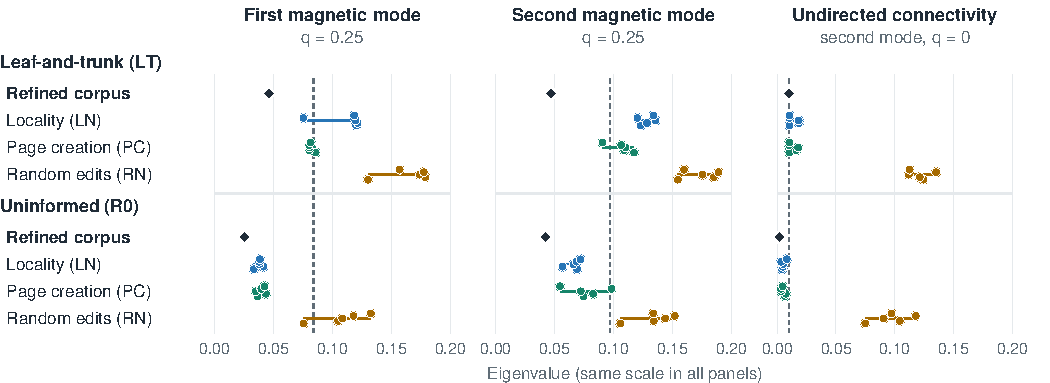
\includegraphics[width=\textwidth]{figures/w02-refinement.pdf}
\caption{Lanes represent refinement styles and their matched controls.
The first magnetic mode is the best-fitting directional pattern; the second
is the next independent pattern. Lower magnetic eigenvalues mean stronger
directional coherence within these patterns, not demonstrated information
flow; lower undirected values mean weaker connectivity. Diamonds show refined
corpora; dots show five controls per row, with segments spanning their range
(not uncertainty). Dashed lines mark original and coincident mapped baselines.
Each graph uses its own LWCC (Table~\ref{tab:refinement-summary}).}
\label{fig:refinement}
\end{figure*}
\begin{table}[t]
\caption{Full-graph pages $N$, links $m$, isolates $I$, mean out-degree $\bar{k}=m/N$ and density $d=m/[N(N-1)]$. LWCC: $n$, $\lambda_1(.25)$ and $F_0$. Area means are LN-standardized LT--R0; rejection threshold $.05$.}
\label{tab:refinement-summary}
\centering
\begin{tabular}{@{}lrrrrrrr@{}}
\toprule
Arm & $n/N$ & $m$ & $I$ & $\bar{k}$ & $d$ (\%) & $\lambda_1$ & $F_0$\\
\midrule
O & 844/1218 & 2494 & 292 & 2.05 & 0.168 & 0.0842 & 0.412\\
LT & 1671/1823 & 5203 & 146 & 2.85 & 0.157 & 0.0462 & 0.314\\
R0 & 1182/1229 & 4502 & 43 & 3.66 & 0.298 & 0.0253 & 0.572\\
\addlinespace
\multicolumn{8}{@{}l@{}}{\textit{Area-paired tests: sample size, mean, $p$}}\\
\multicolumn{8}{@{}l@{}}{Historical (unnormalized): 18, $-0.80$, $0.079$}\\
\multicolumn{8}{@{}l@{}}{Exclude three second-chance areas (unnormalized): 15, $-1.07$, $0.044$}\\
\multicolumn{8}{@{}l@{}}{Normalized (exploratory): 18, $-2.95$, $0.000618$}\\
\bottomrule
\end{tabular}
\end{table}

Both refinements lower LWCC $\lambda_1$, with R0 lowest
(Table~\ref{tab:refinement-summary}); their first two modes fall below their
own LN ranges (Fig.~\ref{fig:refinement}). Ordinary descriptors also separate
edits from nulls. Trophic incoherence falls for LT and rises for R0.

The historical unnormalized test uses area-specific components, LN
standardization and an exact two-sided sign flip, fixed before editing.
It does not reject; excluding second-chance LT areas crosses the threshold
only as a sensitivity result. The smaller normalized $p$-value is exploratory
(Table~\ref{tab:refinement-summary}). Chained areas are not independent realizations.

\begin{table}[t]
\caption{Observed link use: accepted-action shares and trace-level chain. Support is judged at page level. All 1,368 saved traces passed identity/history checks.}
\label{tab:link-use}
\centering
\begin{tabular}{@{}lrr@{}}
\toprule
Measure & LT & R0\\
\midrule
\multicolumn{3}{@{}l@{}}{\textit{Accepted follows}}\\
Added / all accepted & 39/76 & 20/67\\
Mean added-edge menu share & 0.443 & 0.303\\
Added-edge use share & 0.513 & 0.299\\
\addlinespace
\multicolumn{3}{@{}l@{}}{\textit{Trace chain (111 follow-enabled FAQ traces/arm)}}\\
Accepted added-edge follow & 28 & 15\\
First destination-text exposure & 21 & 11\\
Directly supported destination & 7 & 2\\
Cited lines returned by that follow & 7 & 1\\
\bottomrule
\end{tabular}
\end{table}

LT has larger added-edge menu and accepted-follow shares than R0
(Table~\ref{tab:link-use}): greater use accompanies greater availability.
Only a minority of traces reach citation through added-edge use, first exposure
and direct support, more in LT; judged-span overlap is a separate branch.

\begin{figure}[t]
\centering
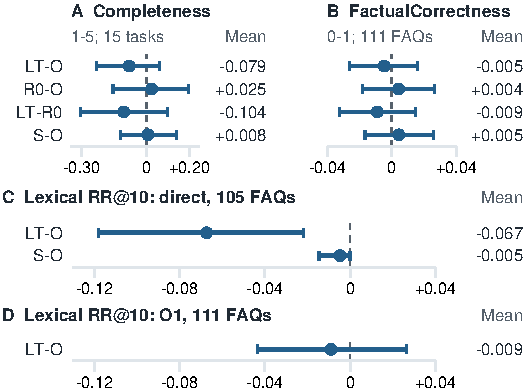
\includegraphics[width=\columnwidth]{figures/w02-answer-intervals.pdf}
\caption{Mean score differences (dots, first minus second) with 95\% intervals
(bars). Positive favors the first arm; including zero means no clear difference,
not equivalence. Metric scales differ; C/D share one. O1 credits moved/derived
content. S--O is replay, not a noise bound.}
\label{fig:answers}
\end{figure}
Primary answer measures show no clear treatment separation
(Fig.~\ref{fig:answers}); the secondary rubric favors R0 over LT but does not
clearly distinguish LT from O. Direct judgments rank LT support lower than O/R0
for lexical and graph-expanded retrieval. The LT--O deficit shrinks under O1,
with an interval spanning zero; the primary replay contrast is much smaller
than the deficit. Embedding retrieval and Recall@5 show no clear separation.
Other O1 gains depend on derived-page credit~\cite{docspectraicsc2027}.

\subsection{A Separate Link-Selection Example}
\label{sec:link-selection-example}
A link-only comparison tests whether magnetic structure changes selection when
semantic assessments tie. Four curated Docker development groups contain
830, 53, 6 and 8 pages. Thirteen candidates wrap existing prose without changing
its words; neither link direction already exists, and endpoints share a baseline
weak component. Each group allows one addition, separately from the LT experiment.

After exposed selector development, Claude Haiku 5.5 and gpt-6.1-sol reviewed
complete source/target pages in isolated requests, blind to prior judgments
and magnetic values. Each scored relationship support, target support and
placement from 0 to 2. Both required every dimension $\geq1$, total $\geq5$,
and no uncertainty or contradiction. Haiku alone sets the admitted semantic
tier; a fixed tie order defines the semantic comparator.

Using the same $W$ and $\theta$ as Section~\ref{sec:magnetic-profile},
page values $e^{i\phi_i}$ of unit magnitude give
\begin{equation}
 E_G(\phi)=\sum_{i<j}2W_{ij}[1-\cos(\phi_i-\phi_j-\theta_{ij})].
 \label{eq:link-phase}
\end{equation}
At $q=.25$, the selector estimates $[F(G+P)-F(G)]/B$ for each candidate $P$,
where $F(G)=\min_\phi E_G(\phi)$ and $B=\sum_{\text{old }i<j}W_{ij}$ stays
fixed for the original group. Unchanged biconnected edge blocks cancel;
changed blocks are solved jointly. Two schedules (seeds 3501/3502), each with
eight L-BFGS-B starts, retain stationary estimates with full-gradient infinity
norm $\leq10^{-7}$. Their extrema measure schedule sensitivity, not error bounds.
A minimum set must have raw envelope spread $\leq10^{-6}$ and every outsider
strictly beyond its upper envelope plus $10^{-6}$; the fixed semantic order
chooses within it. Any unavailable highest-tier option or unresolved overlap
forces whole-tier semantic fallback. Analytic $q=0$ gives the same semantic
choice, without an optimized ordinary-navigation comparator.

All thirteen pass both AI gates. The 53-page language group has eleven options
tied at Haiku 6/6: eight continuous integration and delivery (CI/CD) additions
have raw cost $.194407$, versus $.401924$ for three testing additions.
Here $B=21$. Lower-cost edits create two edge-sharing transitive triangles;
higher-cost edits close two bridges into a triangle. Neither creates a directed cycle.
Restricting the tie order to the eight minima changes .NET
development $\to$ unit tests to C++ development $\to$ CI/CD; cost does not
distinguish C++ from the other seven minima. The Extensions singleton falls
back after nonstationary estimates; Next.js has one option, and the remaining
group has none. Thus only one of four groups is competitive, evaluable and
changed. Actual edits and matched numerical replay were verified.

This is selection behavior on curated, previously inspected examples with
repeated templates, followed by blinded AI support. It supplies neither human
validation nor independent replication. The finite unit-phase cost uses the
magnetic operator's weights and phases; it is not a certified optimum or a
measured decrease in normalized $\lambda_1$, whose eigenvectors allow varying
amplitudes. Retrieval and answer benefit were not tested.

